\documentclass{leaflet}
\usepackage[ngerman]{babel}
\usepackage[utf8]{inputenc}
\usepackage{blindtext}
\usepackage{biolinum}
\renewcommand\rmdefault{\sfdefault}% Verwende serifenlose Schrift
\usepackage{mwe}% Dummy Bilder
\usepackage{xcolor}
\usepackage{framed}
\usepackage{scrextend}

\AddToBackground{1}{\put(0,0){\textcolor{white!20}{\rule{\paperwidth}{\paperheight}}}}% Farbiger Hintergrund für 1. Seite
\begin{document}

{\centering
 
\includegraphics[width=\linewidth]{img/logo}	
}

\vspace{2cm}

{\centering
 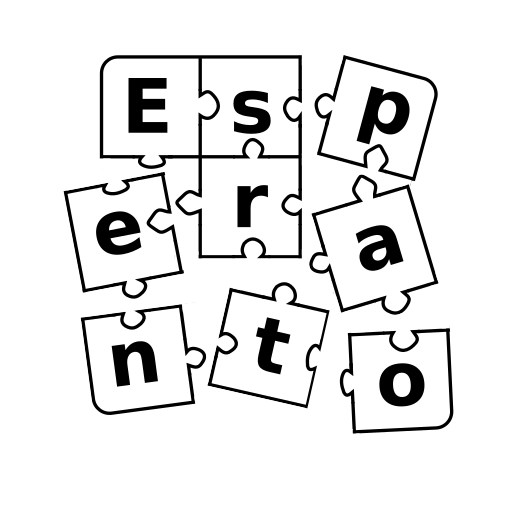
\includegraphics[width=\linewidth]{img/puz}	
}

{
\centering

\Huge
Lingvo kiel ludo

\huge
Eine Sprache wie ein Spiel
}

\thispagestyle{empty}% Keine Seitenzahlen


\clearpage


\begin{center}
{
\Huge \textbf{\textcolor{red}{ESPERANTO}}
}
\end{center}

\vspace{-1cm}

\section{Die regelmäßige Sprache}

\vspace{-.4cm}

\begin{flushright}
\textbf{\large \textcolor{red}{la regula lingvo}}
\end{flushright}

\vspace{-.2cm}

Esperanto ist eine Sprache, die für die Verständigung zwischen Menschen verschiedener Muttersprachen entwickelt wurde. Inzwischen wird Esperanto seit über 130 Jahren und in über 100 Ländern gesprochen. Seinen Erfolg verdankt Esperanto insbesondere seiner schnellen Erlernbarkeit. Der Wortschatz ist verschiedenen Sprachen entnommen; viele Wörter sind international bekannt. Es hat eine einfache, regelmäßige Grammatik. Ein durchdachtes Wortbildungssystem verringert die Zahl der zu lernenden Vokabeln erheblich und fördert den kreativen Umgang mit der Sprache.

Schon nach einigen Wochen kann man alltägliche Gespräche führen und auf internationalen Treffen Freundschaften mit Menschen aus aller Welt schließen oder Menschen in aller Welt besuchen.

Warum Esperanto so überraschend schnell zu lernen ist, wird schon aus dem folgenden kurzen Überlick deutlich:

\vspace{-.4cm}

\section{wie geschrieben so gesprochen}

\vspace{-.2cm}

\begin{flushright}
\textbf{\large \textcolor{red}{kiel skribata tiel parolata}}
\end{flushright}

\vspace{-.2cm}

Für jeden Laut gibt es genau einen Buchstaben und genau einen Laut. Daher gibt es ein paar typische Esperanto-Buchstaben:

\begin{tabular}{llll}
		ĉ & wie in \textbf{Tsch}ad: Ĉado & ĝ & 
		wie in \textbf{Dsch}ungel: \textbf{ĝ}angalo\\
		ĥ & wie in Ya\textbf{ch}t: jaĥto & ĵ & 
		wie in \textbf{J}ournalist: \textbf{ĵ}urnalisto\\
		ŝ & wie in \textbf{Sch}iff: ŝipo & ŭ & 
		wie in \textbf{Au}to: a\textbf{ŭ}to
\end{tabular}


und solche, die von der deutschen Aussprache abweichen:

\begin{tabular}{llll}
c& wie in \textbf{Z}igarre: cigaro&
r& wird gerollt\\
s& wie in Ku\textbf{ss}: kiso&
v& wie in \textbf{w}arm: varma\\
z& wie in Ro\textbf{s}e: rozo& &\\
\end{tabular}

Die Buchstaben q, w, x und y kommen im Esperanto-Alphabet nicht vor.
Die einzige Betonungsregel: Mehrsilbige Wörter werden immer auf der vorletzen Silbe betont, also ho\textbf{te}lo, a\textbf{mi}ko
\clearpage

\vspace{-.6cm}

\section{eine Grammatik ohne Ausnahmen}

\vspace{-.2cm}

\begin{flushright}
\textbf{\large \textcolor{red}{gramatiko sen esceptoj}}
\end{flushright}

\vspace{-.7cm}

\subsection{Artikel:}

\vspace{-.2cm}

Es gibt nur einen bestimmten Artikel: la (der, die, das). Der unbestimmte Artikel (ein, eine) wird nicht übersetzt.

\begin{tabular}{ll}
la tablo - der Tisch  & tablo - ein Tisch
\end{tabular}

\vspace{-.3cm}

\subsection{Haupt- und Eigenschaftswörter}

\vspace{-.1cm}

Alle Hauptwörter (Substantive) enden auf -o und alle \\ Eigenschaftswörter (Adjektive) auf -a:

\begin{tabular}{ll}
ronda tablo -& ein runder Tisch
\end{tabular}

In der Mehrzahl (Plural) wird ein -j an Haupt- und Eigenschaftswort angehängt:

\begin{tabular}{ll}
rondaj tabloj -& runde Tische
\end{tabular}

Im Akkusativ (''Objektfall'') wird ein -n an Haupt- und Eigenschaftswort angehängt:

\begin{tabular}{ll}
	la rondan tablon -& den runden Tisch
\end{tabular}

Eine Reihe von Wörtern wird im Esperanto schematisch gebildet, was das Erlernen erleichtert. Zum Beispiel:

\begin{tabular}{llll}
	kiu - wer   &tiu - dieser   &neniu - niemand  &ĉiu - jeder\\
	kie - wo    &tie - dort     &nenie - nirgendwo&ĉie - überall
\end{tabular}

Die Eigenschaftswörter werden immer durch Vorsetzen von pli (mehr) und plej (am meisten) gesteigert:

\begin{tabular}{ll}
granda - groß  & pli granda (ol) - größer (als)  \\ \multicolumn{2}{l}{la plej granda (el) - am größten (von)}
\end{tabular}

\vspace{-.3cm}

\subsection{Umstandswörter}

\vspace{-.1cm}

Umstandswörter (Adverbien) haben, wie in anderen Sprachen, eine eigene Endung, nämlich -e.
Vergleiche:

\begin{tabular}{ll}
Eva estas bela. & Eva ist schön (Eigenschaftswort)\\
Eva kantas bele. & Eva singt schön (Umstandswort)
\end{tabular}

\vspace{-.2cm}

\subsection{Ja/Nein-Fragen werden mit ĉu eingeleitet:}

\begin{tabular}{ll}
	Ĉu vi komprenas min? -& Verstehst du mich?\\
	Jes, mi komprenas vin. -& Ja, ich verstehe dich.\\
	Ne, mi ne komprenas vin. -& Nein, ich verstehe dich nicht.
\end{tabular}

\clearpage

\subsection{Fürwörter}

\vspace{-.2cm}

Die persönlichen Fürworter (Pronomen) lauten:

\begin{tabular}{ll}
mi - ich & ni - wir\\
vi - du  & vi - ihr\\
li - er (Person) & ili - sie (Mehrzahl)\\
ŝi - sie (Person) & oni - man\\
ĝi - es (Sache) & si - sich
\end{tabular}

Die besitzanzeigenden Fürwörter lassen sich bilden, indem man an die persönlichen Fürwörter ein -a anhängt.

\begin{tabular}{lll}
mia - mein & via - dein & usw.
\end{tabular}

Die vier Fälle werden gebildet wie bei den Hauptwörtern (siehe mittlere Spalte):
mi (ich), de mi (meiner), al mi (mir), min (mich), usw.

\vspace{-.3cm}

\subsection{Zeitwörter}
\hfill\hfill
\vspace{-.7cm}

Auch die Formen der Zeitwörter (Verben) werden vollkommen regelmäßig gebildet. Unregelmäßige Verben gibt es nicht! Drei Endungen genügen für die Bildung von Gegenwart, Vergangenheit und Zukunft:

Gegenwart -as:

\begin{tabular}{ll}
mi amas vin &- ich liebe dich\\
vi amas min &- du liebst mich\\
li amas vin &- er liebt dich\\
ni amas vin &- wir lieben dich, usw.
\end{tabular}


%Vergangenheit -is: \hfill mi amis vin \hfill ich liebte dich \\
%Zukunft -os: \hfill  mi amos vin \hfill ich werde dich lieben \\
%Bedingungsform -us: \hfill  mi amus vin \hfill  ich würde dich lieben\\
%Befehlsform -u: \hfill  amu min! \hfill  liebe mich! \\
%Grundform -i: \hfill  ami \hfill  lieben\\

\begingroup
\setlength{\tabcolsep}{2.5pt} % Default value: 6pt
\renewcommand{\arraystretch}{0.9} % Default value: 1
\begin{tabular}{llr}
Vergangenheit -is: & mi amis vin & ich liebte dich \\
Zukunft -os: & mi amos vin & ich werde dich lieben \\
Bedingungsform -us: & mi amus vin & ich würde dich lieben \\
Befehlsform -u: & amu min! & liebe mich! \\
Grundform -i: & ami & lieben\\
\end{tabular}
\endgroup

\begin{framed}
	\textbf{Hast du Lust bekommen, Esperanto mal hautnah zu sehen und nutzen? 
	Hier ein paar Beispiele, was du für Möglichkeiten hast:} \\
		Suche nach Leuten in deiner Nähe, die Esperanto sprechen: \hfill \textit{\textbf{{\small www.amikumu.com/de/}}}\\
		Finde eine Übernachtungsmöglichkeit im Urlaub mit Esperanto: \hfill \textit{\textbf{{\small www.pasportaservo.org}}}\\
		Fahre auf eines von vielen internationalen Esperantoveranstaltungen: \hfill \textit{\textbf{{\small www.lingvo-internacia.eu/eventoj}}}\\

\end{framed}

\clearpage

\vspace{-.6cm}

\begin{tabular}{lr}
	\textbf{\large{Zahlen mit System}} & \textbf{\large \textcolor{red}{nombroj kun sistemo}}
\end{tabular}

\vspace{-.0cm}

\begingroup
\setlength{\tabcolsep}{5pt} % Default value: 6pt
\renewcommand{\arraystretch}{0.9} % Default value: 1
\begin{tabular}{llllllll}
1 &unu & 6 &ses & 11 &dek unu &  100& cent \\
2 &du  & 7 &sep & 12 &dek du& 200& ducent \\
3 &tri & 8 &ok  & 20 &dudek & 1000& mil \\
4 &kvar& 9 &naŭ & 21 &dudek unu & 2000& dumil \\
5 &kvin& 10 &dek& 30 &tridek& 2001& dumil unu
\end{tabular}
\endgroup

miliono heißt Million. Mit diesen Zahlwörtern kann man schon ganz schön viele Schäfchen zählen!
Bonan nokton! - Gute Nacht! \\
Die Ordnungszahlen werden mit -a gebildet:

\begin{tabular}{lll}
unua - erste/-r/-s & dua - zweite/-r/-s & usw. 
\end{tabular}

\vspace{-.6cm}

\section{Wörter nach dem Baukastenprinzip}

\vspace{-.2cm}

\begin{flushright}
\textbf{\large \textcolor{red}{vortoj laŭ la konstrukesta sistemo}}
\end{flushright}

\vspace{-.1cm}

Mit den Wortbildungssilben lassen sich aus wenigen Grundwörtern viele neue Begriffe ableiten. Hier die wichtigsten dieser Wortbildungssilben:

\textbf{Vorsilben:}

\begin{tabular}{ll}
ek-  &beginnende Handlung; ekiri - losgehen {\footnotesize (iri - gehen)}\\
mis- &falsch; misiri - sich verirren\\
mal- &Gegenteil; malhela - dunkel {\footnotesize (hela - hell)}\\
re-  &wieder, zurück; revidi - wiedersehen {\footnotesize (vidi - sehen)}\\
\end{tabular}

\textbf{Nachsilben}

\begin{tabular}{ll}
-ar-  &Sammelbegriff; ŝiparo - Flotte {\footnotesize(ŝipo - Schiff)}\\
-aĉ-  &Verschlechterung; hundaĉo - Köter {\footnotesize(hundo - Hund)}\\
-ebl- &Möglichkeit; legebla - lesbar {\footnotesize(legi - lesen)}\\
-eg-  &Vergrößerung; ŝnurego - Strick {\footnotesize (ŝnuro - Schnur)}\\
-et-  &Verkleinerung; ŝnureto - Schnürchen \\
-ej-  &Ort, Raum; bakejo - Bäckerei {\footnotesize(baki - backen)}\\
-in-  &weibliches Geschlecht; {\footnotesize (bovino - Kuh)}\\
-iĉ-  &männliches Geschlecht; boviĉo - Stier\\
-ig-  &machen; purigi - reinigen {\footnotesize(pura - sauber)}\\
-iĝ-  &werden; blindiĝi - erblinden {\footnotesize(blinda - blind)}\\
-il-  &Mittel, Werkzeug; skribilo - Stift {\footnotesize(skribi - schreiben)}\\
-ind- &wert, würdig; vidinda - sehenswert {\footnotesize (vidi - sehen)}\\
-ist- &Beruf; instruisto - Lehrer, {\footnotesize (instrui - unterrichten)}\\
-ul-  &Person; fremdulo - Fremder {\footnotesize (fremda - fremd)}
\end{tabular}

\textbf{Rätsel}: Wenn sana gesund heißt, was heißt dann: krank, sanigi, krank werden, malsanulo, malsanulejo, Heilmittel, sanigebla?

\vspace{-.5cm}

\clearpage

\vspace{-.6cm}

\section{einfach Espernto lernen}

\vspace{-.3cm}

\begin{flushright}
\textbf{\large \textcolor{red}{simple lerni Esperanton}}
\end{flushright}

\vspace{-.3cm}

{\centering
	Es gibt sehr viele Möglichkeiten, Esperanto zu lernen.
} 

Auf Wochenendkursen lernst du mit anderen zusammen ein Wochenende lang konzentriert und komprimiert. Falls du in deiner Stadt fünf Leute für einen Kurs findest, schickt die DEJ dir kostenlos eine Lehrperson. 

Aber auch daheim für dich kannst du Esperanto lernen: mit der Website www.lernu.net, per E-Mail-Korrespondenzkurs oder einem Computerkurs. 

Eine der besten Möglichkeiten ist natürlich, einfach auf ein Treffen zu fahren. 

Im Buchhandel gibt es übrigens auch den Sprachführer Esperanto aus der bekannten 'Kauderwelsch'-Reihe.

Kurse im Internet:

{
	\begin{addmargin}[.5em]{.3em}
	www.learn.esperanto.com/ \hfill www.esperanto.de/lernen \\
	www.lernu.net \hfill www.ikurso.net \\
	www.duolingo.com/course/eo/ 
	\end{addmargin}
}

\vspace{-.4cm}

\section{ein paar einfache Ausdrücke}

\vspace{-.3cm}

\begin{flushright}
\textbf{\large{\textcolor{red}{kelkaj simplaj esprimoj}}}
\end{flushright}

\vspace{-.3cm}

{
Saluton! Bonan tagon! \hfill Hallo! Guten Tag!\\
Kiel vi fartas?       \hfill Wie geht es dir/euch/Ihnen?\\
Bone, dankon! Kaj vi? \hfill Gut danke, und dir/Ihnen?\\
Kiel vi nomiĝas?      \hfill Wie heißt du/ihr/heißen Sie?\\
Mia nomo estas...     \hfill Mein Name ist...\\
De kie vi venas?      \hfill Woher kommst du?\\
Mi venas el Germanio. \hfill Ich komme aus Deutschland.
}
	
\begin{framed}
{\centering
\textbf{Deutsche Esperanto-Jugend e.V.} \\
Bundesgeschäftsstelle Esperanto-Laden\\
Katzbachstr. 25 - 10965 Berlin\\
www.esperanto.de\\
}
\end{framed}

\vspace{-.4cm}

{\footnotesize Herausgeber: Deutsche Esperanto-Jugend, 3. Auflage, Berlin 2018 \\
Wir danken dem Bundesministerium für Familie, Senioren, Frauen und Jugend für die freundliche Unterstützung dieser Broschüre. }

%\vspace{-.4cm}

\noindent
\rotatebox{180}{%
	\begin{minipage}{\textwidth}
		\hfill		
		{\scriptsize Auflösung des Rätsels: krank - malsana; sanigi - gesund machen, heilen; krank werden - malsaniĝi; malsanulo - Kranker; malsanulejo - Krankenhaus; Heilmittel - sanigilo; sanigeble - heilbar}
		\hfill
	\end{minipage}%
}%

\end{document}